\subsection{Coverage}
\label{sec:completeness}

The coverage metric provides a quantitative measure of how well a
feed captures the intended threat. A feed with perfect
coverage would include all indicators that belong in a category.
Unfortunately, as discussed above, there is no systematic way for
evaluating the exact accuracy or coverage of a feed since it is unrealistic
to obtain ground truth of all threat activities on the Internet.

However, there are some large-scale threat activities that are
well-collected and well-studied. One example is Internet
scanning. Researchers have long been using ``Internet telescopes'' to
observe and measure network scanning
activities~\cite{benson2015leveraging, durumeric2014internet,
  pang2004characteristics}.  With a large telescope and well-defined
scan filtering logic, one can obtain a comprehensive view of global
scanning activities on the Internet.

To this end, I collected three months of traffic (from January 1st to
March 31st 2018) using the UCSD network telescope~\cite{telescope},
which monitors a largely quiescent /8 network comprising over 16
million IP addresses.  I then used the default parameters of the Bro
IDS~\cite{BroNetwork} to identify likely scanning traffic, namely
flows in which the same source IP address is used to contact 25 unique
destination IP addresses on the same destination port/protocol within
5 minutes. Given the large number of addressed being monitored, any
indiscriminate scanner observed by \ti\ feeds will likely also be seen
in my data.  Indeed, by intersecting against this telescope data we
are able to partially quantify the coverage of each \ti\ scanning feed.


%(u'TS Alien Vault OTX Malicious IPs', 'scan') 0.966922702159 0.0045119148556
%(u'dshield-ips', 'scan') 0.951590802754 0.00826350821018
%(u'TS Packetmail iprep ramnode', 'scan') 0.933286248198 0.00306798601481
%(u'packetmail-ip', 'scan') 0.87635529608 0.00365935255666
%(u'et-ip-reputation', 'scan') 0.627009603999 0.00230524603455
%(u'TS Anomali Labs MHN', 'scan') 0.855805914736 0.0032333616247
%(u'TS Snort IP BlockList', 'scan') 0.0862598022503 1.2237504915e-05
%(u'FB Basecamp Streetcred', 'scan') 0.153300600109 1.3591853285e-05
%(u'TS Analyst', 'scan') 0.523206751055 1.19956569917e-05

The scanners I collected from the telescope consist of 20,674,149 IP addresses.
The total number of IPs in all the scan feeds during this period is
425,286, which covers only 1.7\% (363,799 shared IPs) of all the telescope scan IPs.
On the other hand, telescope scanners intersect with 85\% of all IPs in scan feeds.
When looking at each feed, {\feedTSAlienVault}, {\feeddshield}
{\feedpacketmail}, {\feedTSLabScan} and {\feedTSramnode} all have over 85\% of their
data intersected with telescope scanners; the other four, though, have less than 65\%
of their data shared (and the rate for {\feedTSSnort} is only 8\%).


To further understand how well each scan feed detects scanning
activities, I measure how different sizes of scanners in the
telescope are covered by each feed. Here, \emph{scanner size} means how
many IPs a scanner has scanned in the telescope within a
day. Figure~\ref{fig:caida_coverage_cdf} shows the coverage rate of
each feed over different sizes of scanners, ranging from 1,000 to
1 million. \textbf{Y} axis is the proportion of scanners of a given size or 
larger that are covered by each feed. (There are 7,212,218 scanners from the 
telescope whose sizes
are over 1K, 271,888 that are over 100K and 17,579 are over 1 million.)


\begin{figure}
\centering
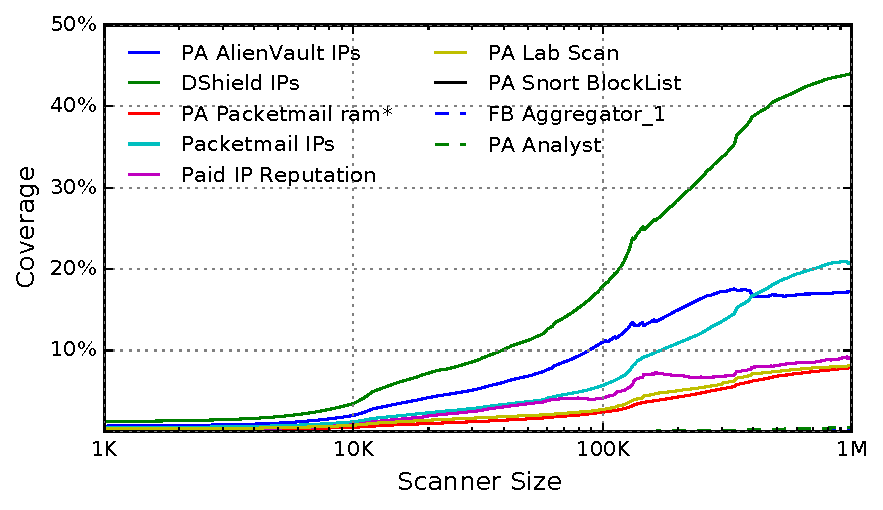
\includegraphics[width=0.8\textwidth]{data_character/images/caida_coverage_cdf.pdf}
\caption{The coverage of each feed on different sizes of scanners.}
\label{fig:caida_coverage_cdf}
\end{figure}

\finding\
The union of all the scan IPs in the feeds covers less than
2\% of the scanners collected by the telescope. Even if I only look
at the scanners with sizes larger than 10,000, the overall coverage is still
around 10\%, suggesting the coverage capability of scan feeds
is very limited. The graph shows that, as the scanner size increases, the coverage of
each feed over the datasets also increases, and large feeds cover more percent
of telescope scanners than small feeds. This trend aligns with the intuition that
scan feeds tend to capture more extensive scanners.

It is surprising that the small scan feeds in my collection have a smaller percentage of their
IPs shared with telescope scanners. This contradicts the idea that small feeds
would contain a larger percentage of extensive scanners (that would most likely also be observed by the telescope).

%Using another metric, the volume of scanners in the
%telescope is over 20 times larger than that of the scan feeds, yet the
%telescope scanners only cover 25.9\% of all of the scanning feeds'
%data. The overall volume of scanning activities is so extensive that
%even a /8 telescope will miss many of them, particularly if scanners
%are selective in targets (avoiding or focusing on certain IP ranges)
%or rate limits (falling below scanner labeling thresholds). The
%coverage curve based on scanner sizes showed that scan feeds are
%better at capturing large scanners, which is intuitive, but that a
%larger feed does not necessarily mean better coverage.


%\begin{table}
%\small
%\caption{Intersection between scan feeds and telescope scanners.
%\textit{Volume} contains the total amount of IPs in each feed from
%Jan. 2016 to July 2016. \textit{Intersection} is the proportion
%of each feed's IPs that overlap with the telescope data.}
%\centering
% \resizebox{0.7\linewidth}{!}{
%\begin{tabular}{l r r }
%\toprule
%Feed & Volume & Intersection \\
%\midrule
%{PA Snort BlockList}     & 312,533   & 18.2\% \\
%{\feedetiprep}           & 293,484   & 22.1\% \\
%{\feedpacketmail}        & 50,723    & 83.6\% \\
%{PA Packetmail ramnode}  & 11,452    & 76.1\% \\
%{\feedalienvault}        & 8,695     & 35.1\% \\
%{PA Malicious IPs}       & 7,960     & 63.3\% \\
%{PA Packetmail CARISIT}  & 5,955     & 71.5\%\\
%{PA SANS Top IPs}        & 3,087     & 77.4\%\\
%{PA Analyst}             & 444       & 52.0\%\\
%{PA Shockpot IPs}        & 156       & 50.0\%\\
%{PA SANS IPs}            & 129       & 63.6\%\\
%{FB Aggregator}          & 103       & 37.9\%\\
%\midrule
%Total & 675,243 & 25.9\%\\
%\bottomrule
%\end{tabular}
%}
%\label{tab:caida_ip_overlap}
%\end{table}
